\section{Generator of synthetic images}

For the purposes of this thesis and training the neural network, a large amount of data is required. To train the network through supervised learning, data also needs to be labeled. 

Unfortunately, instruments available at The Department of Astronomy and Astrophysics are incapable of producing such a large amount of data. Acquired images are also unlabeled and the process of labeling them would be considerably time-consuming.  

Furthermore, the astronomical images required for the thesis should contain features like galaxies and cosmic rays. These features are present in the ground-based images but only in a limited amount. To obtain images with a sufficient amount of these features images need to be acquired through space-based observations of the sky. 

The best option is therefore to generate synthetic images. For the purpose of this thesis the Department of Astronomy and Astrophysics has provided their own generator - starGen. 

\subsection{starGen.R}
The generator \cite{thesisKyselica} is implemented in R language and generates a single FITS image. 
The dimensions of the image can be adjusted using parameters $dimX$ and $dimY$. The generator is only capable of generating stars and their amount is set by parameter $starCount$. 

As mentioned in Section \ref{sec:features} stars can either appear as points or streaks. The script provides the option to choose PSF as either Gaussian or Cauchy and the streak is generated using multiple Gaussian PSFs. This option is specified using parameter $method$, which has 3 possible values (gauss, Cauchy, line). The full width at half maximum of PSF is defined by the $fwhm$ parameter. 
The script also contains parameters to control the maximum and minimum brightness of objects which are defined using parameters $briMax$ and $briMin$, respectively. 

If the method is set to display stars as streaks, additional parameters need to be taken into an account. $Length$ specifies the half-length of the object, where the unit of measurement is $\sigma$ of the Gaussian function. The parameter $\sigma$ is computed from $fwhm$ as:

\begin{equation}
  \sigma = fwhm / 2.355   
\end{equation}


Another required parameter is $alpha$, which defines the slope of the streak in degrees (from 0 to 90) in the anti-clockwise direction. % preco iba od 0 do 90 a nie 180
The script can also generate a sky background noise, which can be approximated using Gaussian noise. The mean value of the Gaussian distribution is specified using parameter $gaussM$ and the standard deviation by $gaussS$. 
The script contains additional parameters, however, we have decided to only mention the ones that are the most relevant for this thesis. 

An example of two images generated by the starGen.R is displayed in the Figure \ref{fig:stargenImages}. Images show two types of appearances (streak, point) of stars as well as different amounts of generated stars. 

\begin{figure}[!h]
    \centering
    \begin{subfigure}{.35\textwidth}
        \centering
        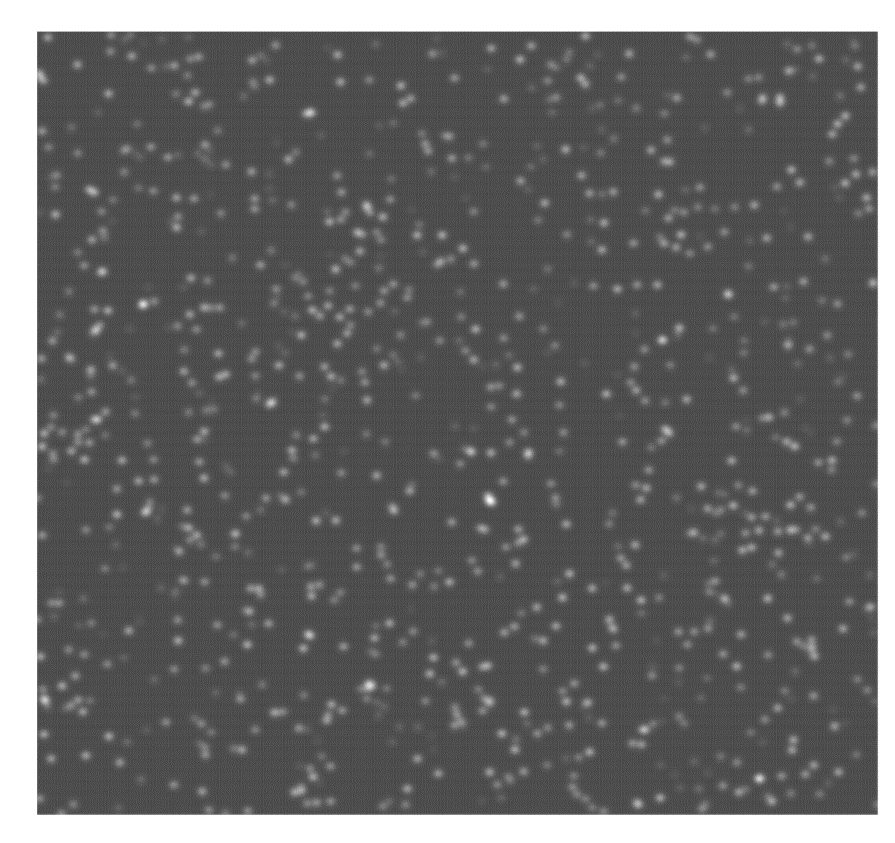
\includegraphics[width=\textwidth]{images/stargenRimage.png}
        \label{fig:stargenImg1}
    \end{subfigure}
    \begin{subfigure}{.35\textwidth}
        \centering
        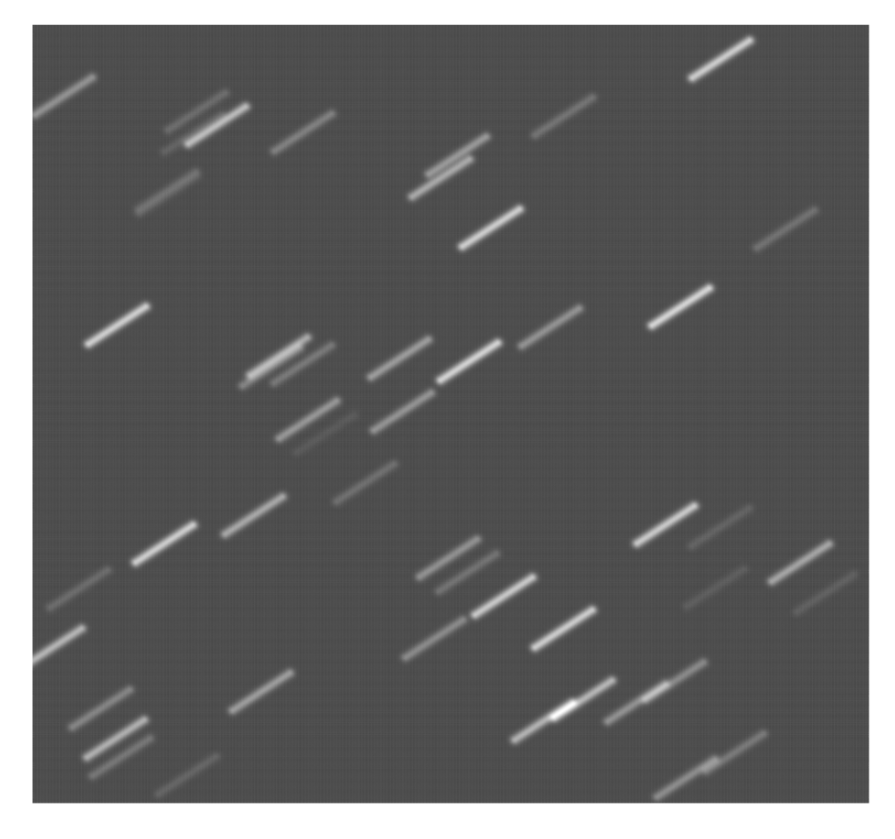
\includegraphics[width=\textwidth]{images/starGenRimage2.png}
        \label{fig:stargenImg2}
    \end{subfigure}
    \caption[Examples of  images generated by starGen.R script.]
    {Examples of  images generated by starGen.R script. 
    (Left) Generated image containing 1000 point-like stars with fwhm of 1. (Right) Generated image containing 50 streak-like stars with fwhm of 1 and lenght of the streak 10.
    Source: \cite{thesisKyselica}.}
    \label{fig:stargenImages}
\end{figure}

\subsection{starGen.py}
Some parts of the starGen script were later converted to Python by Daniel Kyselica \cite{thesisKyselica}. The script was modified to train a neural network to identify tracklets on astronomical images. 

Instead of a single FITS image, the new code is now able to generate a series of 8 images, as depicted in Figure \ref{img:danoStargen1}. Each image now also contains stars and a moving object. 
Since data required for the neural network were just positions of the object, the script is also producing TSV files containing positions of stars and objects on each image. 
As the priority was not the visual part of the generator, the option to display stars as streaks or use the Cauchy function as PSF was not added to the new script. 


\begin{figure}[h]
    \centering
    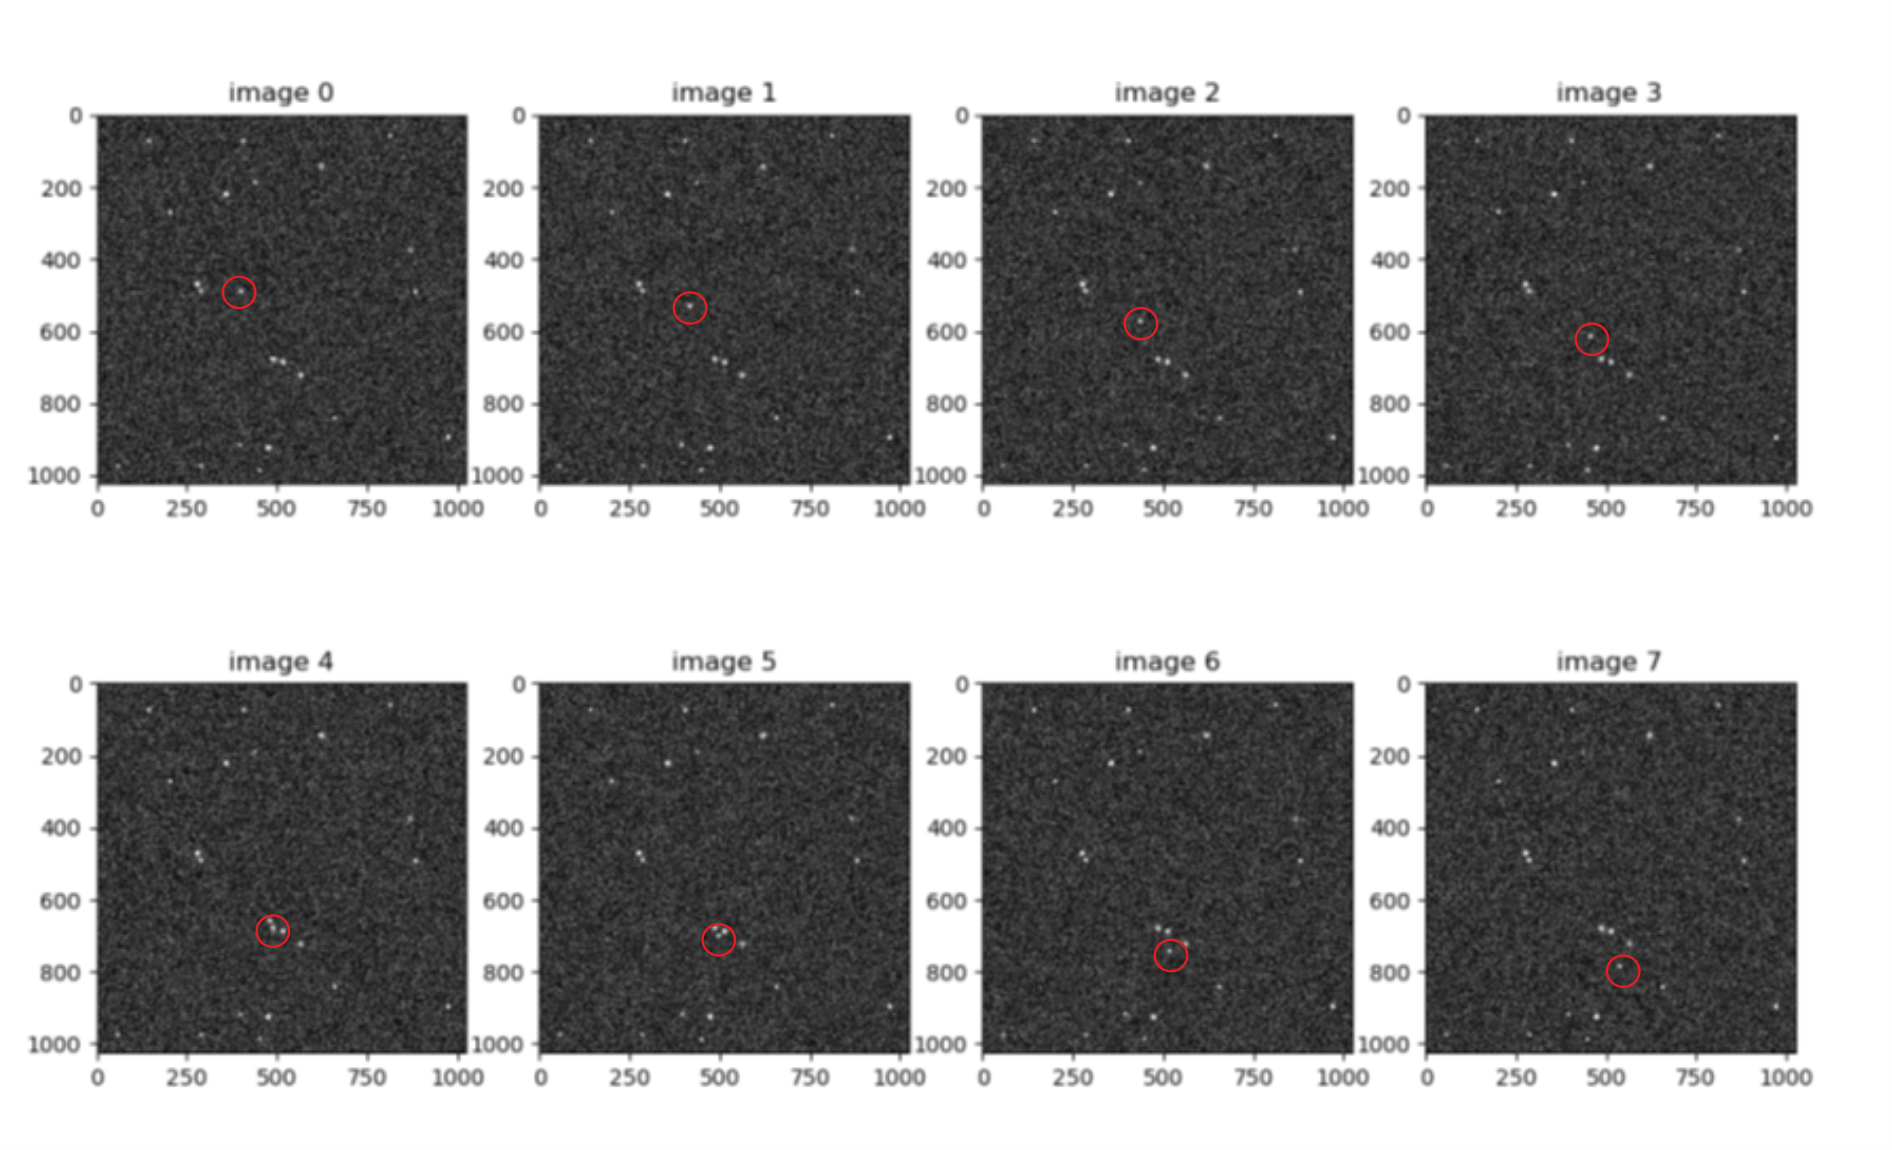
\includegraphics[width=\textwidth]{images/danostargenRed.png}
    \caption[An example of a series of images generated by starGen.py script.]
    {An example of a series of images generated by starGen.py script. The Series show point-like stars, which stay at the same position in all the images. There is also a moving object which is highlighted in the red circle, moving downwards. }
    \label{img:danoStargen1}
\end{figure}
